\documentclass[a4paper, 12pt]{article}
\usepackage[total={17cm,25cm}, top=2.5cm, left=2.5cm, right=2.5cm,  includefoot]{geometry}
\usepackage[utf8]{inputenc}
\usepackage{array}
\usepackage{multirow}
\usepackage{hhline}
\usepackage{gensymb}
\usepackage{graphicx}
\graphicspath{ {} }
\usepackage[czech]{babel}
\usepackage{enumitem}
\usepackage{pdfpages}
\usepackage{amsmath}
\usepackage{verbatim}
\usepackage{listings}
\usepackage{hyperref}
\usepackage{amssymb}


\pagestyle{empty} % vypne číslování stránek




\usepackage[OT2,OT1]{fontenc}
\newcommand\cyr
{
\renewcommand\rmdefault{wncyr}
\renewcommand\sfdefault{wncyss}
\renewcommand\encodingdefault{OT2}
\normalfont
\selectfont
}
\DeclareTextFontCommand{\textcyr}{\cyr}
\def\cprime{\char"7E }
\def\cdprime{\char"7F }
\def\eoborotnoye{\char’013}
\def\Eoborotnoye{\char’003}
\setlength{\parindent}{1em} 
%\setlength{\parskip}{0.5ex}


\begin{document}

\begin{titlepage}
\begin{center}
\Huge
\vspace*{4.5cm}
Algoritmy v digitální kartografii\\
\vspace{0.2cm}

\Large  
Množinové operace s polygony\\
\vspace{0.2cm}

\normalsize  
Zimní semestr 2018/2019\\
%(oprava: 24. 11. 2018)
\vspace{14cm}
\end{center}

\begin{flushright}
\Large
Tereza Kulovaná \\
Markéta Pecenová \\
\end{flushright}

\end{titlepage}


\pagestyle{plain}     % zapne obyčejné číslování
\setcounter{page}{1}  % nastaví čítač stránek znovu od jedné

\tableofcontents
\newpage

\section{Zadání}
Zadání úlohy bylo staženo ze stránek předmětu \href{https://web.natur.cuni.cz/~bayertom/index.php/teaching/algoritmy-v-digitalni-kartografii}{155ADKG}.

\begin{figure}[h!]
	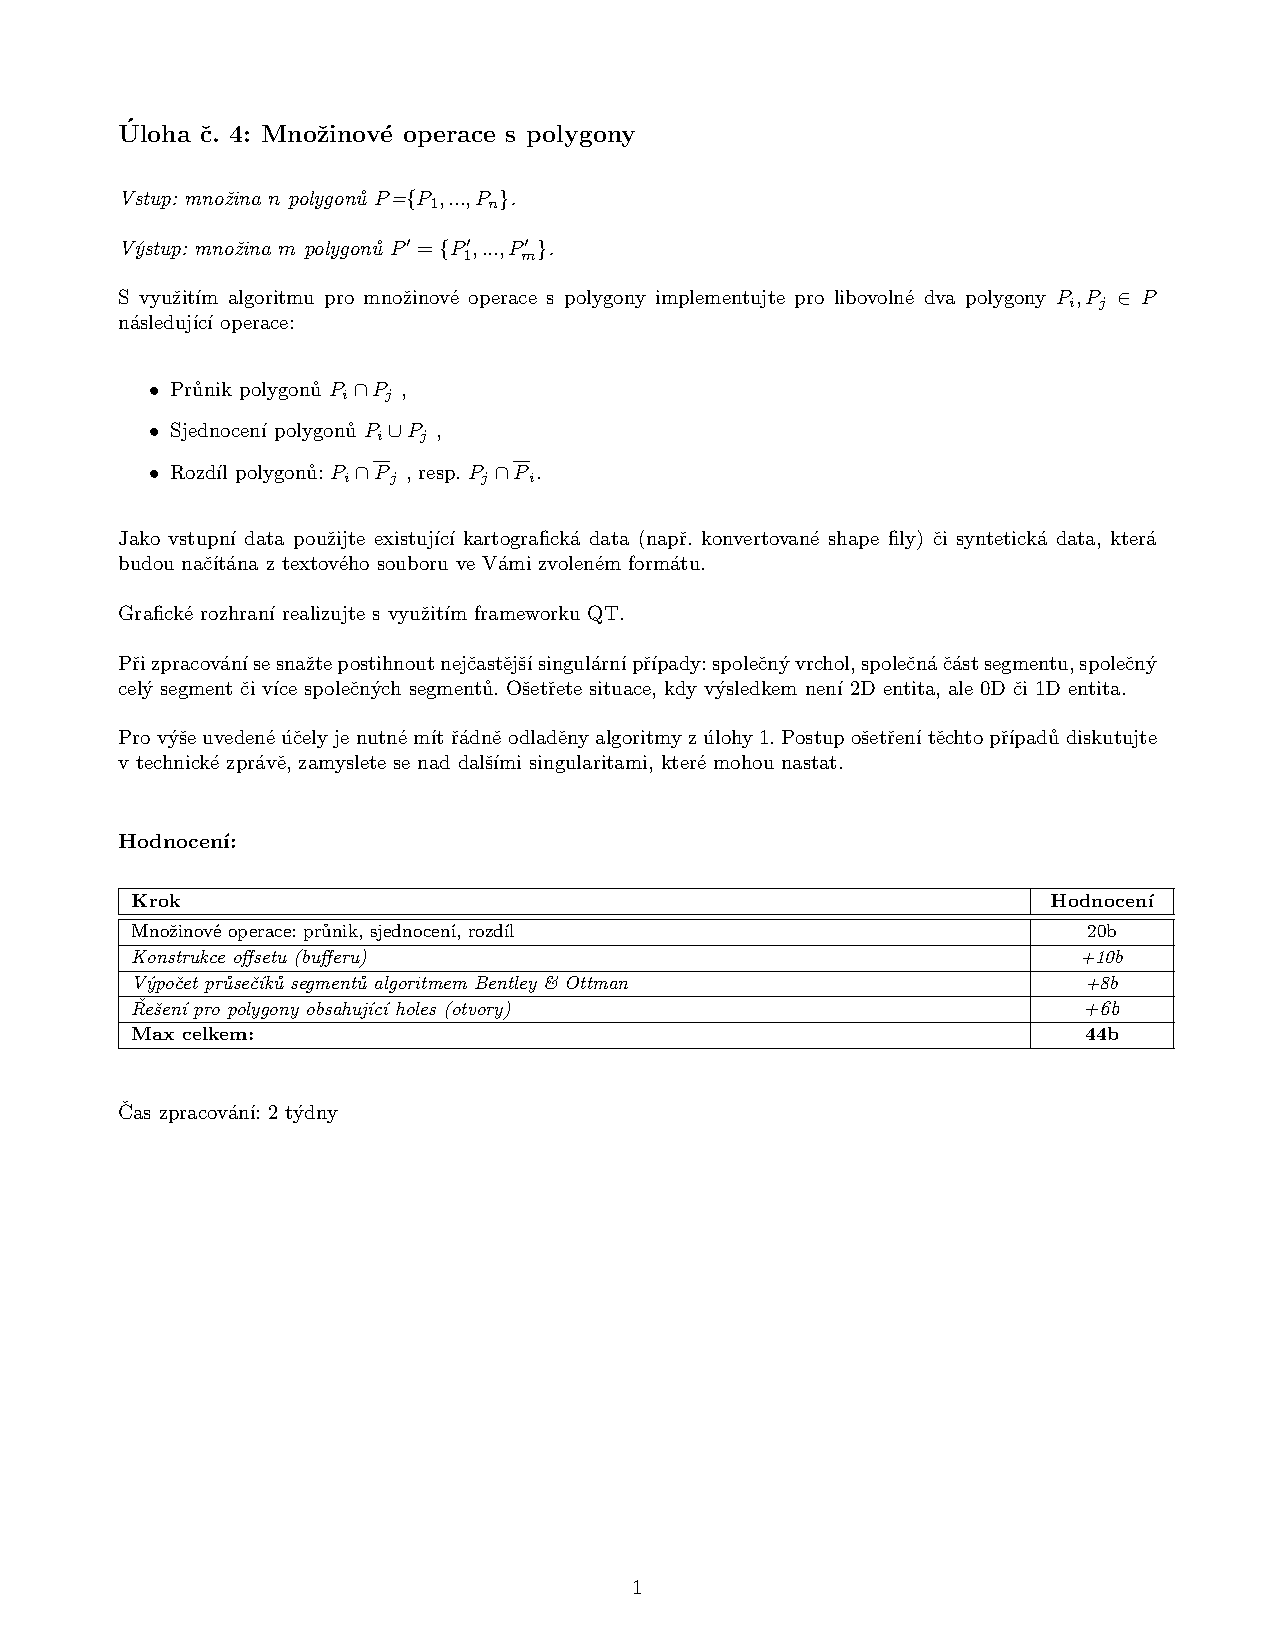
\includegraphics[clip, trim=0cm 8.5cm 0cm 3cm, width=1.0\textwidth]{./pictures/zadani04.pdf}
\end{figure}

V rámci této úlohy nebyly implementovány žádné bonusové úlohy.
\clearpage

\section{Popis a rozbor problému}
Úloha \textbf{Množinové operace s polygony} se zabývá vytvořením aplikace, která nad libovolnými dvěma vstupními polygony provede zvolenou množinovou operaci. \\

Mějme vstupní polygony $A$ a $B$. Množinové operace, které nad nimi lze vykonat, jsou následující:
\begin{enumerate}
\item Průnik (Intersection): $\longrightarrow A \cap B$
\item Sjednocení (Union) $\longrightarrow A \cup B$
\item Rozdíl (Difference) $\longrightarrow A$\textbackslash $B$ nebo $B$\textbackslash $A$
\end{enumerate}

\begin{figure}[h!]
	\centering
	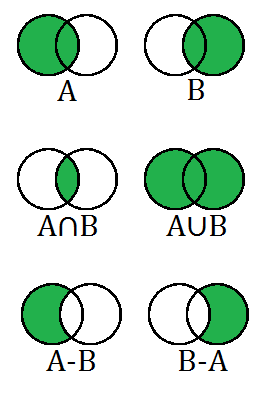
\includegraphics[width=6cm]{./pictures/operations.png}
	\caption{Ukázka množinových operací [\href{http://www.efgh.com/math/algebra/sets.htm}{Zdroj}]}
\end{figure}

\section{Algoritmy}
Tato kapitola se zabývá popisem algoritmů, které byly v aplikaci implementovány. Vzhledem k jejich složitosti je popis výsledného algoritmu rozdělen do jednotlivých fází. Vý\-sled\-ný algoritmus, který spojuje všechny kroky dohromady, se nazývá \textit{BooleanOper}. Vstupní polygony $A$ a $B$ jsou reprezentovány kruhovými seznamy s orientací proti směru hodinových ručiček (CCW). Body, které tvoří oba polygony, mají nově vytvořený datový typ \texttt{QPointFB}.

\subsection{Výpočet průsečíků}
\subsubsection{computePolygonIntersections}
Průsečíky $b_{ij}$ jsou ukládány do proměnné $M$ datového typu \texttt{map}, která funguje na principu hashování. Spolu s výsledkem je ukládán i tzv. klíč, který na něj odkazuje. Za klíč byl zvolen parametr $\alpha$.\\

Po nalezení každého nového průsečíku je nutné aktualizovat stávající seznamy bodů obou polygonů. K tomu slouží lokální procedura \textit{ProcessIntersection}. Parametr $t$ reprezentuje směrnice $\alpha$ nebo $\beta$, parametr $i$ index daného bodu.\\

Zjednodušený zápis algoritmů lze zapsat způsobem uvedeným níže:

\begin{enumerate}
\item[] Postupně pro všechny $p_i \in A$:
\subitem Vytvoř mapu M 
\subitem Postupně pro všechny $p_j \in B$:
\subitem \hspace {0.5cm} Podmínka ($\exists$ průsečík $b_{ij}$):
\subitem \hspace {1cm} Přidej: M[$\alpha_{i}] \leftarrow b_{ij}$
\subitem \hspace {1cm} Zpracuj průsečík pro $B$: \textit{ProcessIntersection($b_{ij}, \beta, B, j$)}
\subitem Podmínka ($M \neq \emptyset$):
\subitem \hspace {0.5cm} Postupně pro všechny $b_{ij} \in M$:
\subitem \hspace {1cm} Zpracuj průsečík pro $A$: \textit{ProcessIntersection($b_{ij}, \alpha, A, i$)}
\end{enumerate}
~\\

Lokální procedura \textit{ProcessIntersection($b, t, P, i$)}:
\begin{enumerate}
\item  Podmínka ($|t| < \epsilon)$: 
\subitem Průsečíkem je počáteční bod: $P[i] \leftarrow inters$
\item  Podmínka ($(|t-1| < \epsilon)$:
\subitem Průsečíkem je koncový bod: $P[(i+1)\%n] \leftarrow inters$
\item  Jinak:
\subitem Inkrementace: $i = i+1$
\subitem $P \leftarrow (b,i)$
\end{enumerate}

\subsubsection{setPositions}
Všechny vrcholy polygonu A, resp. B (včetně nalezených průsečíků) jsou následně ohodnoceny, zda leží uvnitř, vně nebo na hraně polygonu B, resp. A. Pro všechny hrany $e_i$ jsou vypočteny jejich středy $\bar{p}$, pro které se následně určuje jejich pozice (ohodnocení $g$) vůči druhému polygonu. Tato informace je uložena do počátečního bodu hrany $e_i$ do parametru pozice. K určení pozice bodu vůči polygonu byl použit algoritmus \textit{GetPositionWinding} z úlohy č.~1. Nejprve jsou zpracovány všechny hrany prvního polygonu a stejný postup je analogicky aplikován i pro druhý polygon. \\

Zjednodušený zápis algoritmů lze zapsat způsobem uvedeným níže:
\begin{enumerate}
\item [] Postupně pro všechny $p_i \in A$:
\subitem $\bar{p} = \frac{p_i(x,y)+p_{i+1}(x,y)}{2}$
\subitem pozice = \textit{GetPositionWinding($\bar{p},B$)}
\subitem $p_i[pozice]$ = pozice
\end{enumerate}

\subsection{Fragmenty}
Sousedící vrcholy se stejným ohodnocením jsou uloženy do samostatných fragmentů $f$. Seznam bodů každého fragmentu začíná průsečíkem a končí bodem s jiným ohodnocením. Pro odlišení je orientace vrcholů ve fragmentech po směru hodinových ručiček (CW). 

\subsubsection{createFragments}
Do metody vstupuje polygon $P$ o velikosti $n$, ohodnocení vrcholů $g$ a seznam fragmentů $F$. Algoritmus obsahuje lokální proceduru \textit{createFragmentFromVertices}, která ze sousedících bodů o stejném ohodnocení vytváří fragment $f$. $i_s$ je index počátečního bodu fragmentu, $i$ je index přidávaného bodu a $g$ ohodnocení.\\

Zjednodušený zápis algoritmů lze zapsat způsobem uvedeným níže:
\begin{enumerate}
\item Inicializace: $i = n-1;~i_s = -1$
\item Dokud ($i > 0$)
\subitem Podmínka ($P[i] =$ průsečík $\land~g(P[i]) = g$)
\subitem \hspace {0.5cm} $i_s = i$; $i--$ 
\item Podmínka ($i_s < 0$) $\rightarrow$ žádný bod neexistuje, ukonči proces
\item Inicializace: $i = i_s$
\item Proveď: 
\subitem Podmínka ($P[i] =$ průsečík $\land~g(P[i]) = g$)
\subitem \hspace {0.5cm} Vytvoř fragment $f = \emptyset$ 
\subitem \hspace {0.5cm} Podmínka (\textit{createFragmentFromVertices} vytvořen)
\subitem \hspace {1cm} Je-li potřeba, prohoď orientaci
\subitem \hspace {1cm} Přidej $f$ do seznamu fragmentů $F$: $F[f[0]] \leftarrow f$
\subitem Jinak inkrementace: $i = (i+1)\%n$
\item[] Dokud ($i \neq i_s$)
\end{enumerate}
~\\

Lokální procedura \textit{createFragmentFromVertices($i_s, P, g, i, f$)}:
\begin{enumerate}
\item[] Opakuj:
\subitem Přidej bod do fragmentu: $f \leftarrow P[i]$
\subitem Inkrementace: $i = (i+1)\%n$
\subitem Podmínka ($i = i_s$) $\rightarrow$ return FALSE
\subitem Podmínka ($g(P[i]) \neq g$)
\subitem \hspace {0.5cm} Přidej bod do fragmentu: $f \leftarrow P[i]$
\subitem \hspace {0.5cm} Return TRUE
\end{enumerate}

\subsubsection{mergeFragments}
Algoritmus spojuje jednotlivé fragmenty $f$ do výstupních polygonů. Metoda má na vstupu seznam fragmentů $F$ a seznam polygonů $C$, do kterého jsou ukládány výsledné polygony. Metoda nejprve spojí jednotlivé fragmenty do oblastí a ty jsou následně lokální procedurou \textit{createPolygonFromFragments} převedeny na polygony. Počáteční bod fragmentu je značen jako $s$, $n$ značí následující bod.

\begin{enumerate}
\item[] Postupně pro všechna $f \in F$:
\subitem Vytvoř: $P = \emptyset$
\subitem Najdi startovní bod fragmentu: $s = f.first$
\subitem Podmínka ($f$ nebyl ještě zpracován)
\subsubitem Podmínka (\textit{createPolygonFromFragments})
\subsubitem Přidej: $C \leftarrow P$
\end{enumerate}
~\\

Lokální procedura \textit{createPolygonFromFragments($s, F, P$)}:
\begin{enumerate}
\item[] Inicializace: $n = s$
\subitem Opakuj:
\subsubitem Nalezni další fragment: $f = F.find(n)$
\subsubitem Podmínka (fragment s daným počátečním bodem $\nexists$) $\rightarrow$ return FALSE
\subsubitem Označ fragment za zpracovaný: $f.second.first \leftarrow$ TRUE
\subsubitem Nalezni další bod: $n \leftarrow f.second.second.back()$
\subsubitem Přidej fragment bez počátečního bodu: $P \leftarrow f.second.second - {f.second.second[0]}$
\subsubitem Podmínka ($n = s$) $\rightarrow$ return TRUE
\end{enumerate}

\subsection{BooleanOper}
Tento algoritmus spojuje všechny výše uvedené kroky. Na vstupu jsou polygony $A$ a $B$ a typ zvolené množinové operace.
\begin{enumerate}
\item Podmínka (orientace $A \lor B \neq$ CCW) $\rightarrow$ prohoď orientaci
\item \textit{computePolygonIntersections($A,B$)}
\item \textit{setPositions($A,B$)}
\item Vytvoř mapu fragmentů $F$
\item Zvolení ohodnocení: $pos1 = (oper \equiv intersection \lor oper \equiv DiffAB?Inner:Outer)$
\subitem \hspace {2.8cm} $pos2 = (oper \equiv intersection \lor oper \equiv DiffBA?Inner:Outer)$
\item Prohození: $swap1 = (oper \equiv DiffAB? : true : false)$
\subitem \hspace {1.2cm} $swap2 = (oper \equiv DiffBA? : true : false)$
\item \textit{CreateFragments (A, pos1, swap1, F)}
\item[] \textit{CreateFragments (B, pos2, swap2, F)}
\item \textit{MergeFragments (A,B,C)}

\end{enumerate}


\section{Vstupní data}
Seznam bodů vstupních polygonů je uložen v textovém souboru \textit{polygons.txt}. Pro vykreslení polygonů v aplikaci je nutno tento soubor do aplikace nahrát pomocí tlačítka \textsl{Load polygon file}. K vygenerování souřadnic bodů byla použita online aplikace ze stránek mobilefish.com. Struktura souboru s polygony je následující:\\

\noindent
\textsl{První řádek}: počet bodů $n$ v polygonu A\\
\textsl{Sloupec 2}: souřadnice X bodu polygonu A\\
\textsl{Sloupec 3}: souřadnice Y bodu polygonu A\\
...\\
\textsl{(n+2)-tý řádek}: počet bodů $m$ v polygonu B\\
\textsl{Sloupec 2}: souřadnice X bodu polygonu B\\
\textsl{Sloupec 3}: souřadnice Y daného polygonu B\\

Po úspěšném/neúspěšném nahrání souboru je uživatel upozorněn hláškou. Uživatel nemůže kliknout na žádné jiné tlačítko, nejsou-li nahrána data (tlačítka jsou zašedivělá). Po nahrání vstupního souboru jsou data vykreslena a uživatel získá možnost zvolit, jaký typ množinové operace bude nad daty prováděn rozbalením nabídky \textsl{Boolean Operations}. Výpočet se provede stisknutím tlačítka \textsl{Boolean Operations}. 

\section{Výstupní data}
Vstupní polygony a nad nimi provedená množinová operace jsou zobrazeny v grafickém okně aplikace. Polygon A je vykreslen zelenou barvou, polygon B modrou barvou a výsledek operace je zobrazen červeně. Tlačítkem \textsl{Clear results} má uživatel možnost smazat výsledek operace při zachování vykreslení původních polygonů. Tlačítko \textsl{Clear All} maže veškerá vykreslená data.

\section{Aplikace}
V následují kapitole je představen vizuální vzhled vytvořené aplikace tak, jak ji vidí prostý uživatel.\\

\begin{figure}[h!]
	\centering
	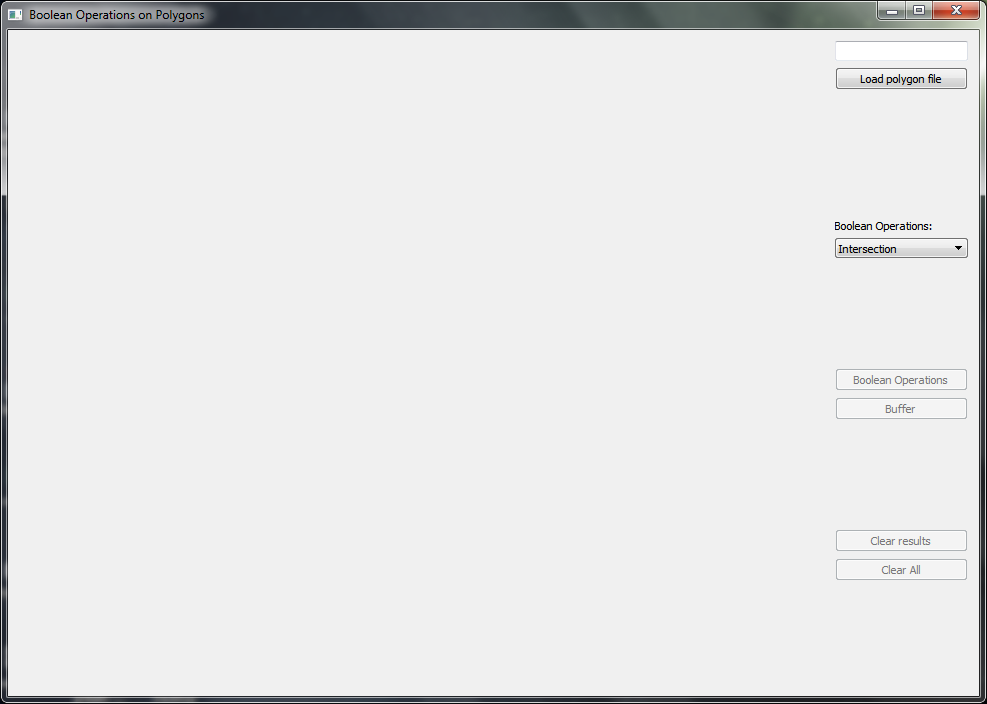
\includegraphics[width=15cm]{./pictures/app_default.png}
	\caption{Výchozí vzhled aplikace po spuštění}
\end{figure}

\begin{figure}[t]
	\centering
	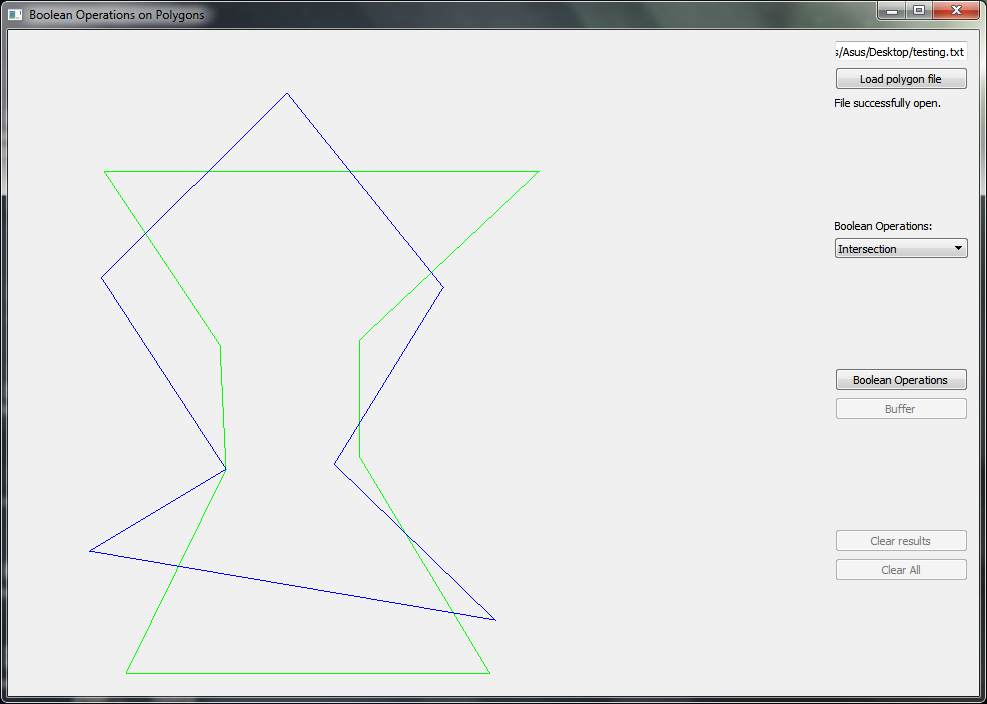
\includegraphics[width=14.5cm]{./pictures/app_load_data.png}
	\caption{Aplikace po nahrání vstupních dat}
\end{figure}
\vspace{2cm}

\begin{figure}[b]
	\centering
	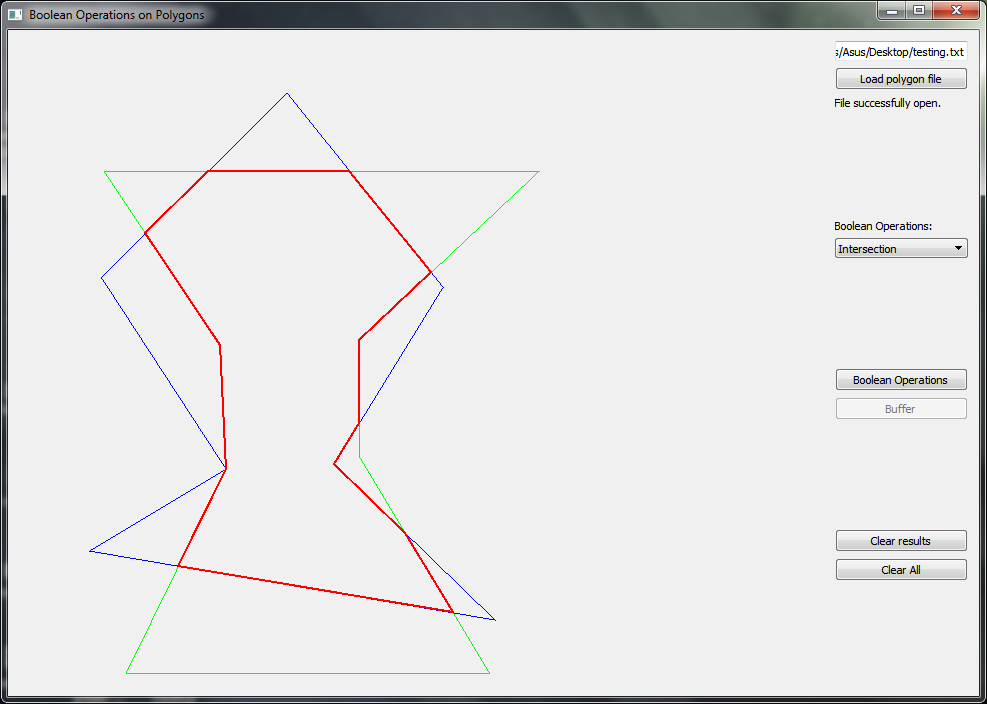
\includegraphics[width=14.5cm]{./pictures/app_intersection.png}
	\caption{Průnik polygonů $A \cap B$}
\end{figure}

\begin{figure}[h!]
	\centering
	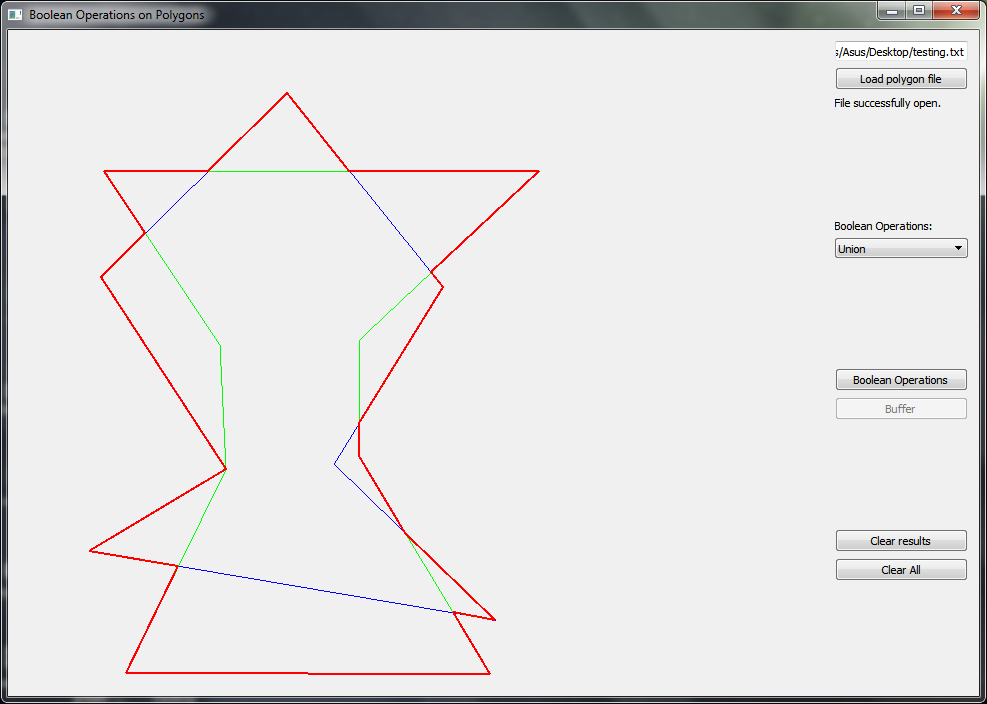
\includegraphics[width=14.5cm]{./pictures/app_union.png}
	\caption{Sjednocení polygonů $A \cup B$}
\end{figure}

\begin{figure}[h!]
	\centering
	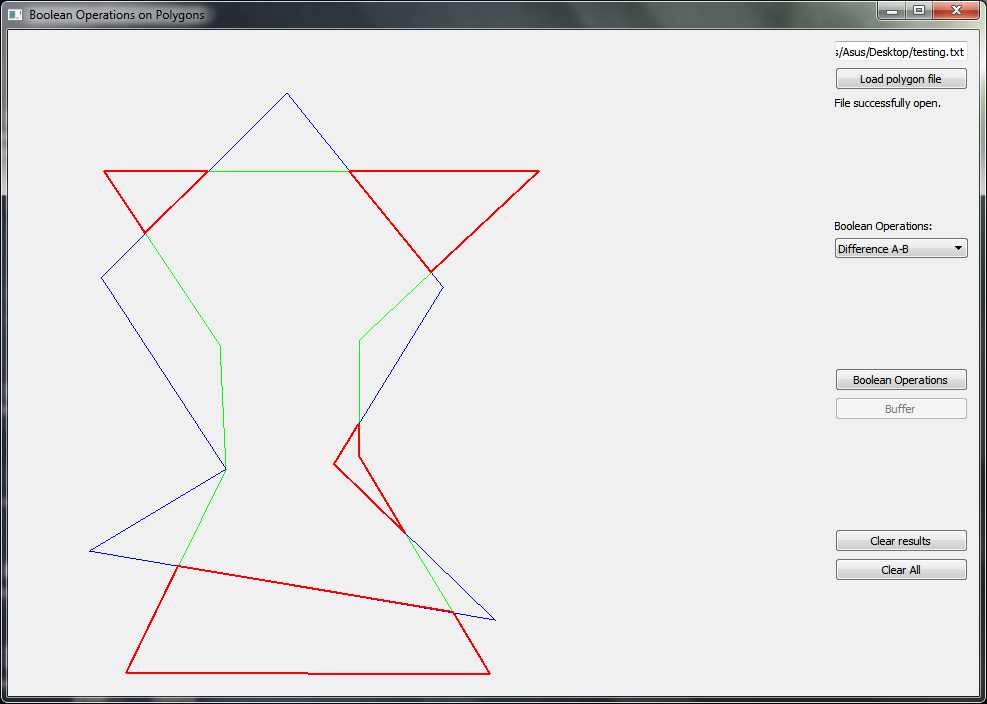
\includegraphics[width=14.5cm]{./pictures/app_diffAB.png}
	\caption{Rozdíl polygonů $A$\textbackslash$B$}
\end{figure}
\clearpage

\begin{figure}[t!]
	\centering
	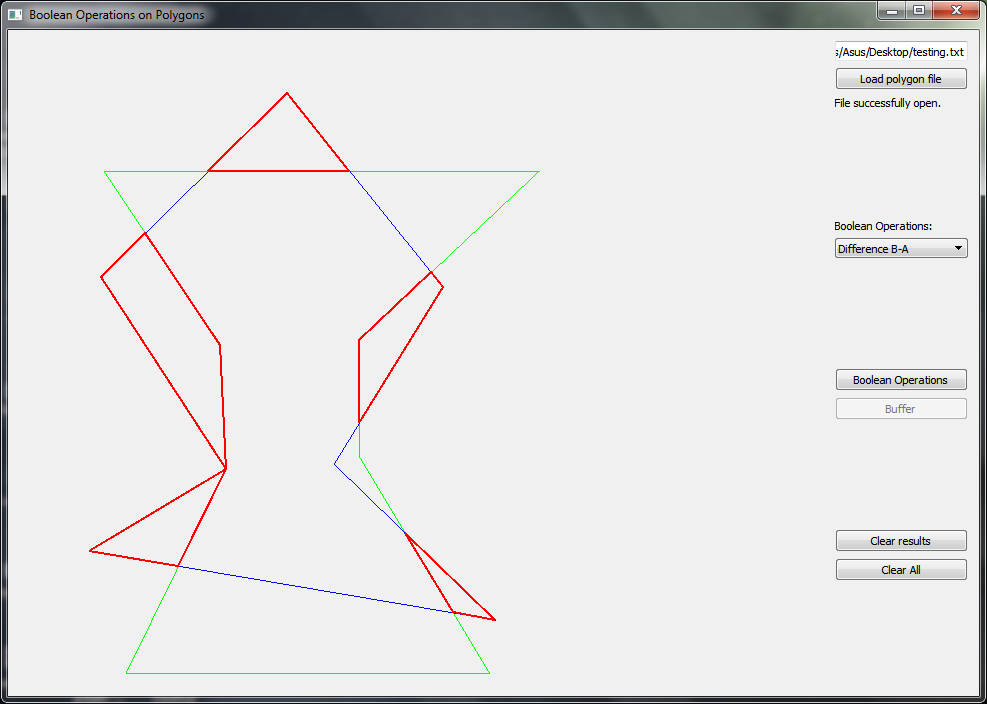
\includegraphics[width=14.5cm]{./pictures/app_diffBA.png}
	\caption{Rozdíl polygonů $B$\textbackslash$A$}
\end{figure}
~\\
\clearpage


 
\section{Dokumentace}
Tato kapitola obsahuje dokumentaci k jednotlivým třídám.

\subsection{Algorithms}
Třída \textit{Algorithms} obsahuje metody pro realizaci množinových operací. Dále obsahuje pomocné algoritmy k jejich fungování.

\subsubsection*{getPositionWinding}
Metoda \textbf{getPositionWinding} určuje polohu bodu $q$ vzhledem k polygonu $pol$ za použití algoritmu \textsl{Winding Number}. Na vstupu je bod $q$ a vektor bodů polygonu třídy \texttt{QPointFB}. Návratová hodnota typu \texttt{TPointPolygon} vrací polohu bodu $q$ vůči polygonu $pol$.\\

\textbf{Input}:
\begin{itemize}
\item \texttt{QPointFB} $q$
\item \textsl{vector} $\textless$\texttt{QPointFB}$\textgreater$ $pol$
\end{itemize}

\textbf{Output}:
\begin{itemize}
\item \texttt{INSIDE} $\rightarrow q$ se nachází uvnitř polygonu $pol$
\item \texttt{OUTSIDE} $\rightarrow q$ se nachází vně polygonu $pol$
\item \texttt{ON} $\rightarrow q$ se nachází na hraně polygonu $pol$
\end{itemize}

\subsubsection*{getPointLinePosition}
Metoda \textbf{getPointLinePosition} určuje polohu bodu $q$ vzhledem k přímce tvořené dvěma body. Na vstupu jsou 3 body typu \texttt{QPointFB}, návratová hodnota je nově definovaný typ \texttt{TPosition}.\\

\textbf{Input}:
\begin{itemize}
\item \texttt{QPointFB} $q$
\item \texttt{QPointFB} $a$
\item \texttt{QPointFB} $b$
\end{itemize}

\textbf{Output}:
\begin{itemize}
\item \texttt{LEFT} $\rightarrow$ bod se nachází vlevo od přímky
\item \texttt{RIGHT} $\rightarrow$ bod se nachází vpravo od přímky
\item \texttt{ON} $\rightarrow$ bod se nachází na přímce
\end{itemize}

\subsubsection*{get2LinesAngle}
Metoda \textbf{get2LinesAngle} počítá úhel mezi dvěma přímkami. Na vstupu jsou 4 body typu \texttt{QPointFB}, návratová hodnota typu \texttt{double} vrací velikost úhlu v radiánech. Body $p_1$ a $p_2$ definují první přímku, zbylé dva body druhou přímku.\\

\textbf{Input}:
\begin{itemize}
\item \texttt{QPointFB} $p_1$ 
\item \texttt{QPointFB} $p_2$ 
\item \texttt{QPointFB} $p_3$
\item \texttt{QPointFB} $p_4$
\end{itemize}

\textbf{Output}:
\begin{itemize}
\item \texttt{double} 
\end{itemize}

\subsubsection*{get2LinesPosition}
Metoda \textbf{get2LinesPosition} určuje vzájemnou polohu dvou přímek. Pokud se přímky protínají, metoda vypočte jejich průsečík $p_{intersection}$. Na vstupu jsou 4 body typu \texttt{QPointFB}, návratová hodnota je nově definovaný typ \texttt{T2LinesPosition}. Body $p_1$ a $p_2$ definují první přímku, další dva body druhou přímku.\\

\textbf{Input}:
\begin{itemize}
\item \texttt{QPointFB} $p_1$ 
\item \texttt{QPointFB} $p_2$ 
\item \texttt{QPointFB} $p_3$
\item \texttt{QPointFB} $p_4$
\item \texttt{QPointFB} $p_{intersection}$
\end{itemize}

\textbf{Output}:
\begin{itemize}
\item \texttt{PARALLEL} $\rightarrow$ přímky jsou rovnoběžné
\item \texttt{COLINEAR} $\rightarrow$ přímky jsou kolineární
\item \texttt{INTERSECTING} $\rightarrow$ přímky se protínají v průsečíku $p_{intersection}$
\item \texttt{NONINTERSECTING} $\rightarrow$ přímky se neprotínají
\end{itemize}

\subsubsection*{computePolygonIntersections}
Metoda \textbf{computePolygonIntersections} počítá průsečíky dvou polygonů $A$ a $B$. Na vstupu jsou dva vektory bodů polygonů, návratová hodnota je typu \texttt{void}.\\

\textbf{Input}:
\begin{itemize}
\item \textsl{vector} $\textless$\texttt{QPointFB}$\textgreater$ $polA$
\item \textsl{vector} $\textless$\texttt{QPointFB}$\textgreater$ $polB$
\end{itemize}

\subsection*{processIntersection}
Metoda \textbf{processIntersection} slouží k aktualizování seznamu bodů (tzv. map) polygonu po přidání nově nalezeného průsečíku. Na vstupu jsou čtyři parametry: průsečík $b$, směrnice přímky $t$, vektor bodů polygonu $poly$ a index $i$ aktuálního bodu. Návratová hodnota je typu \texttt{void}.\\

\textbf{Input}:
\begin{itemize}
\item \texttt{QPointFB} $b$
\item \texttt{double} $t$
\item \textsl{vector} $\textless$\texttt{QPointFB}$\textgreater$ $poly$
\item \texttt{int} $i$
\end{itemize}

\subsubsection*{setPositions}
Metoda \textbf{setPositions} určuje pozici vrcholů prvního polygonu vzhledem k druhému polygonu, tzv. je ohodnocuje. Informace o pozici, která je datového typu \texttt{TPointPolygon}, je ukládána do parametru \textit{pos} daného bodu. Na vstupu jsou dva vektory bodů polygonu, návratová hodnota typu \texttt{void}.\\

\textbf{Input}:
\begin{itemize}
\item \textsl{vector} $\textless$\texttt{QPointFB}$\textgreater$ $polA$
\item \textsl{vector} $\textless$\texttt{QPointFB}$\textgreater$ $polB$
\end{itemize}

\subsubsection*{createFragments}
Metoda \textbf{createFragments} vytváří ze sousedních bodů o stejném ohodnocení jednotlivé fragmenty $f$ a ukládá je do seznamu (mapy) fragmentů. Na vstupu je vektor bodů polygonu, ohodnocení (pozice) hledaných bodů, orientace fragmentu a seznam se vzniklými fragmenty. Návratová hodnota je typu \texttt{void}.\\

\textbf{Input}:
\begin{itemize}
\item \textsl{vector} $\textless$\texttt{QPointFB}$\textgreater$ $pol$
\item \texttt{TPointPolygon} $pos$
\item \texttt{bool} $swap$
\item \textsl{map} $\textless$\texttt{QPointFB}, \textsl{pair} $\textless$\texttt{bool},\textsl{vector} $\textless$\texttt{QPointFB}$\textgreater \textgreater \textgreater$ $fragments$
\end{itemize}

\subsubsection*{createFragmentFromVertices}
Metoda \textbf{createFragmentFromVertices} je lokální procedurou metody \textbf{createFragments}, která zajišťuje vytváření fragmentů $f$. Na vstupu je index $i_s$ počátečního bodu fragmentu, vektor bodů polygonu a fragmentu, pozice (ohodnocení) bodů a index $i$ daného bodu. Návratová hodnota typu \texttt{bool} vrací, zda byl fragment vytvořen či nikoli.\\ 

\textbf{Input}:
\begin{itemize}
\item \texttt{int} $i_s$ 
\item \textsl{vector} $\textless$\texttt{QPointFB}$\textgreater$ $pol$
\item \texttt{TPointPolygon} $pos$
\item \texttt{int} $i$ 
\item \textsl{vector} $\textless$\texttt{QPointFB}$\textgreater$ $fr$
\end{itemize}

\textbf{Output}:
\begin{itemize}
\item 0 $\rightarrow$ fragment nebyl vytvořen 
\item 1 $\rightarrow$ fragment byl vytvořen 
\end{itemize}

\subsubsection*{mergeFragments}
Metoda \textbf{mergeFragments} spojuje fragmenty do jednotlivých oblastí a následně do polygonů, které ukládá do seznamu polygonů. Na vstupu je seznam fragmentů \textit{FR} a sez\-nam polygonů $res$. Návratová hodnota je typu \texttt{void}.\\ 

\textbf{Input}:
\begin{itemize}
\item \textsl{map} $\textless$\texttt{QPointFB}, \textsl{pair} $\textless$\texttt{bool},\textsl{vector} $\textless$\texttt{QPointFB}$\textgreater \textgreater \textgreater$ \textit{FR}
\item \textsl{vector} $\textless$\textsl{vector} $\textless$\texttt{QPointFB}$\textgreater \textgreater$ $res$
\end{itemize}

\subsubsection*{createPolygonFromFragments}
Metoda \textbf{createPolygonFromFragments} je lokální procedurou metody \textbf{mergeFragments} a vytváří z fragmentů polygony. Na vstupu je index $start$, seznam fragmentů \textit{FR} a vektor bodů polygonu. Návratová hodnota typu \texttt{bool} vrací, zda byl z fragmentu vytvořen polygon či nikoli.\\

\textbf{Input}:
\begin{itemize}
\item \texttt{int} $start$ 
\item \textsl{map} $\textless$\texttt{QPointFB}, \textsl{pair} $\textless$\texttt{bool},\textsl{vector} $\textless$\texttt{QPointFB}$\textgreater \textgreater \textgreater$ \textit{FR}
\item \textsl{vector} $\textless$\texttt{QPointFB}$\textgreater$ $pol$
\end{itemize}

\textbf{Output}:
\begin{itemize}
\item 0 $\rightarrow$ polygon nebyl vytvořen 
\item 1 $\rightarrow$ polygon byl vytvořen 
\end{itemize}

\subsubsection*{getPolygonOrientation}
Metoda \textbf{getPolygonOrientation} slouží k získání orientace bodů v polygonu za využití l'Huilierových vzorců. Na vstupu je vektor bodů polygonu, návratová hodnota typu \texttt{double} vrací plochu polygonu.\\

\textbf{Input}:
\begin{itemize}
\item \textsl{vector} $\textless$\texttt{QPointFB}$\textgreater$ $pol$
\end{itemize}

\textbf{Output}:
\begin{itemize}
\item \texttt{double} $< 0 \rightarrow$ CW orientace
\item \texttt{double} $> 0 \rightarrow$ CCW orientace
\end{itemize}

\subsubsection*{BooleanOper}
Metoda \textbf{BooleanOper} spojuje výše uvedené algoritmy. Na vstupu jsou dva vektory bodů polygonu, metoda vrací vektor vektoru bodů \texttt{QPointFB}, který obsahuje výsledek zvolené množinové operace.\\

\textbf{Input}:
\begin{itemize}
\item \textsl{vector} $\textless$\texttt{QPointFB}$\textgreater$ $polA$
\item \textsl{vector} $\textless$\texttt{QPointFB}$\textgreater$ $polB$
\end{itemize}

\textbf{Output}:
\begin{itemize}
\item \textsl{vector} $\textless$\textsl{vector} $\textless$\texttt{QPointFB}$\textgreater \textgreater$
\end{itemize}

\subsubsection*{resetIntersections}
\textbf{resetIntersections} je pomocná metoda, která pro všechny body v polygonu nastaví, že nejsou průsečíky. Na vstupu je vektor bodů polygonu, návratová hodnota je typu \texttt{void}.\\

\textbf{Input}:
\begin{itemize}
\item \textsl{vector} $\textless$\texttt{QPointFB}$\textgreater$ $pol$
\end{itemize}

\subsection{Draw}
Třída \textit{Draw} obsahuje metody, které nahrávají a vykreslují vstupní polygony. Dále zajišťuje vykreslení a smazání všech operací, kterou jsou nad polygony prováděny.

\subsubsection*{paintEvent}
Metoda \textbf{paintEvent} vykresluje vstupní polygony a výsledek množinové operace.

\subsubsection*{drawPol}
Metoda \textbf{drawPol} vykresluje vstupní polygon. Na vstupu je vektor bodů polygonu. 

\subsubsection*{loadPolygon}
Metoda \textbf{loadPolygon} slouží k načtení vstupních dat do aplikace. Součástí metody je i kontrola, zda se soubor úspěšně nahrál. Návratová hodnota typu \textsl{QString} vrací hlášku, zda byly polygony úspěšně nahrány či nikoli.

\subsubsection*{setAB}
Metoda \textbf{setAB} slouží k převedení nahraných polygonů do kreslící plochy.

\subsubsection*{clearAll}
Metoda \textbf{clearAll} slouží k vymazání všech vykreslených dat.

\subsubsection*{clearResults}
Metoda \textbf{clearResults} slouží k vymazání výsledku množinové operace. Vstupní polygony zůstávají nedotčené.

\subsubsection*{setRes}
Metoda \textbf{setRes} slouží k převedení výsledného vektoru vektoru bodů do kreslící plochy.

\subsubsection*{setA}
Metoda \textbf{setA} slouží k převedení vektoru bodů polygonu A do kreslící plochy.

\subsubsection*{getA}
Metoda \textbf{getA} slouží k získání vektoru bodů polygonu.

\subsubsection*{setB}
Metoda \textbf{setB} slouží k převedení vektoru bodů polygonu B do kreslící plochy.

\subsubsection*{getB}
Metoda \textbf{getB} slouží k získání vektoru bodů polygonu B.

%\subsubsection*{setBuffer}
%Metoda \textbf{setBuffer} slouží k vykreslení orientace trojúhelníků.


\subsection{QPointFB}
Třída \textit{QPointFB} slouží k definování nového datového typu \texttt{QPointFB}, který je odvozen od typu \texttt{QPointF} a který navíc obsahuje směrnice přímek \textsl{alfa} a \textsl{beta}, informaci, zda bod je průsečíkem, a polohu bodu vůči druhému polygonu. Defaultně je nastaveno, že bod není průsečíkem, leží na hraně druhého polygonu a hodnoty obou směrnic jsou rovny nule.

\subsubsection*{getAlfa}
Metoda \textbf{getAlfa} slouží k získání směrnice \textsl{alfa}.

\subsubsection*{setAlfa}
Metoda \textbf{setAlfa} slouží k nastavení směrnice \textsl{alfa}. 

\subsubsection*{getBeta}
Metoda \textbf{getBeta} slouží k získání směrnice \textsl{beta}.

\subsubsection*{setBeta}
Metoda \textbf{setBeta} slouží k nastavení směrnice \textsl{beta}. 

\subsubsection*{getInters}
Metoda \textbf{getInters} slouží k získání informace, zda bod je průsečíkem (\textit{true}) či nikoli (\textit{false}).

\subsubsection*{setInters}
Metoda \textbf{setInters} slouží k nastavení informace, zda bod je průsečíkem či nikoli. 

\subsubsection*{getPosition}
Metoda \textbf{getPosition} slouží k získání pozice (ohodnocení) bodu.

\subsubsection*{setPosition}
Metoda \textbf{setPosition} slouží k nastavení pozice (ohodnocení) bodu. 


\subsection{Types}
Třída \textit{Types} slouží k definování nových datových typů výčtového typu.

\subsubsection*{TPointPolygon}
Datový typ \textbf{TPointPolygon} definuje polohu bodu $q$ vůči polygonu $P$.\\ 
\begin{itemize}
\item \texttt{INSIDE} $\rightarrow q \in P$
\item \texttt{OUTSIDE} $\rightarrow q \notin P$
\item \texttt{ON} $\rightarrow q$ leží na $P$
\end{itemize}

\subsubsection*{TBooleanOperation}
Datový typ \textbf{TBooleanOperation} definuje množinovou operaci, která je nad polygony $A$ a $B$ prováděna.\\ 
\begin{itemize}
\item \texttt{INTERSECTION} $\rightarrow A \cap B$ 
\item \texttt{UNION} $\rightarrow A \cup B$
\item \texttt{DIFFAB} $\rightarrow A$\textbackslash $B$
\item \texttt{DIFFBA} $\rightarrow B$\textbackslash $A$
\end{itemize}

\subsubsection*{T2LinesPosition}
Datový typ \textbf{T2LinesPosition} definuje polohu dvou přímek $a$ a $b$.\\  
\begin{itemize}
\item \texttt{PARALLEL} $\rightarrow a \parallel b$
\item \texttt{COLINEAR} $\rightarrow a = b$
\item \texttt{INTERSECTING} $\rightarrow a \cap b \neq \emptyset$
\item \texttt{NONINTERSECTING} $\rightarrow a \cap b = \emptyset$
\end{itemize}

\subsubsection*{TPointLinePosition}
Datový typ \textbf{TPointLinePosition} definuje polohu bodu $q$ a přímky $a$.\\   
\begin{itemize}
\item \texttt{LEFT} $\rightarrow$ bod $q$ leží vlevo od přímky $a$
\item \texttt{RIGHT} $\rightarrow$ bod $q$ leží vpravo od přímky $a$
\item \texttt{COL} $\rightarrow$ bod $q$ leží na přímce $a$
\end{itemize}




\subsection{Widget}
Metody třídy \textit{Widget} slouží pro práci uživatele s aplikací. Metody na vstupu nemají žádné parametry a návratové hodnoty jsou typu \texttt{void}.

\subsubsection*{on\_load\_button\_clicked}
Metoda \textbf{on\_load\_button\_clicked} načítá data z textového souboru. Uživatel sám vyhledává cestu k požadovanému souboru.

\subsubsection*{on\_operation\_button\_clicked}
Metoda \textbf{on\_operation\_button\_clicked} nad vstupními polygony provede zvolenou mno\-ži\-no\-vou operaci.

\subsubsection*{on\_clear\_res\_button\_clicked}
Metoda \textbf{on\_clear\_button\_clicked} vymaže výsledek množinové operace z kreslící plochy. 

\subsubsection*{on\_clear\_all\_button\_clicked}
Metoda \textbf{on\_contours\_button\_clicked} vrací aplikaci do výchozí polohy smazáním všeho, co bylo vykresleno. 

%\subsubsection*{on\_buffer\_button\_clicked}
%Metoda \textbf{on\_slope\_button\_clicked} vykreslí nad vstupními polygony buffer o zvolené šířce.


\clearpage
\section{Závěr}
V rámci úlohy \textit{Množinové operace s polygony} byla vytvořena aplikace, která nad dvěma vstupními polygony aplikuje zvolenou množinovou operaci. Implementace algoritmů byla často dost náročná a nad naše síly. Nepodařilo se nám tedy naplnit všechny cíle této úlohy, jako je například ošetření singulárních případů či dodělání bufferu, který byl vytvořen na poslední hodině, ale který obsahoval chybu, kterou se nám nepodařilo nalézt.\\

Do budoucna by jistě bylo vhodné ošetřit právě singulární případy, např. mají-li oba polygony právě jeden společný vrchol nebo celou hranu. Dále by se dal ošetřit případ, má-li jeden (nebo oba) polygony v sobě díru (pro představu, vypadají jako donut).
\clearpage

\section{Zdroje}
\begin{enumerate}
\item  \textsl{BAYER, Tomáš}. Množinové operace s polygony [online][cit. 4. 1. 2019].\\
Dostupné z: \href{https://web.natur.cuni.cz/~bayertom/images/courses/Adk/adk9.pdf}{https://web.natur.cuni.cz}

\item  \textsl{Elementary Set Theory} [online] [cit. 4. 1. 2019].\\
Dostupné z: \href{http://www.efgh.com/math/algebra/sets.htm}{http://www.efgh.com/}

\item \textsl{Record XY mouse coordinates} [online][cit. 5. 1. 2019].\\
Dostupné z: \href{https://mobilefish.com/services/record_mouse_coordinates/record_mouse_coordinates.php}{https://mobilefish.com/}\\
\end{enumerate}

\end{document}
